\documentclass[12pt]{article}

\usepackage{fancyhdr}
\usepackage{gensymb}
\usepackage{amsmath}
\usepackage{epsfig}

\lhead[\fancyplain]{Luke Palmer}
\chead[\fancyplain]{2006-10-19}
\rhead[\fancyplain]{PHYS 4810}
\pagestyle{fancyplain}

\begin{document}
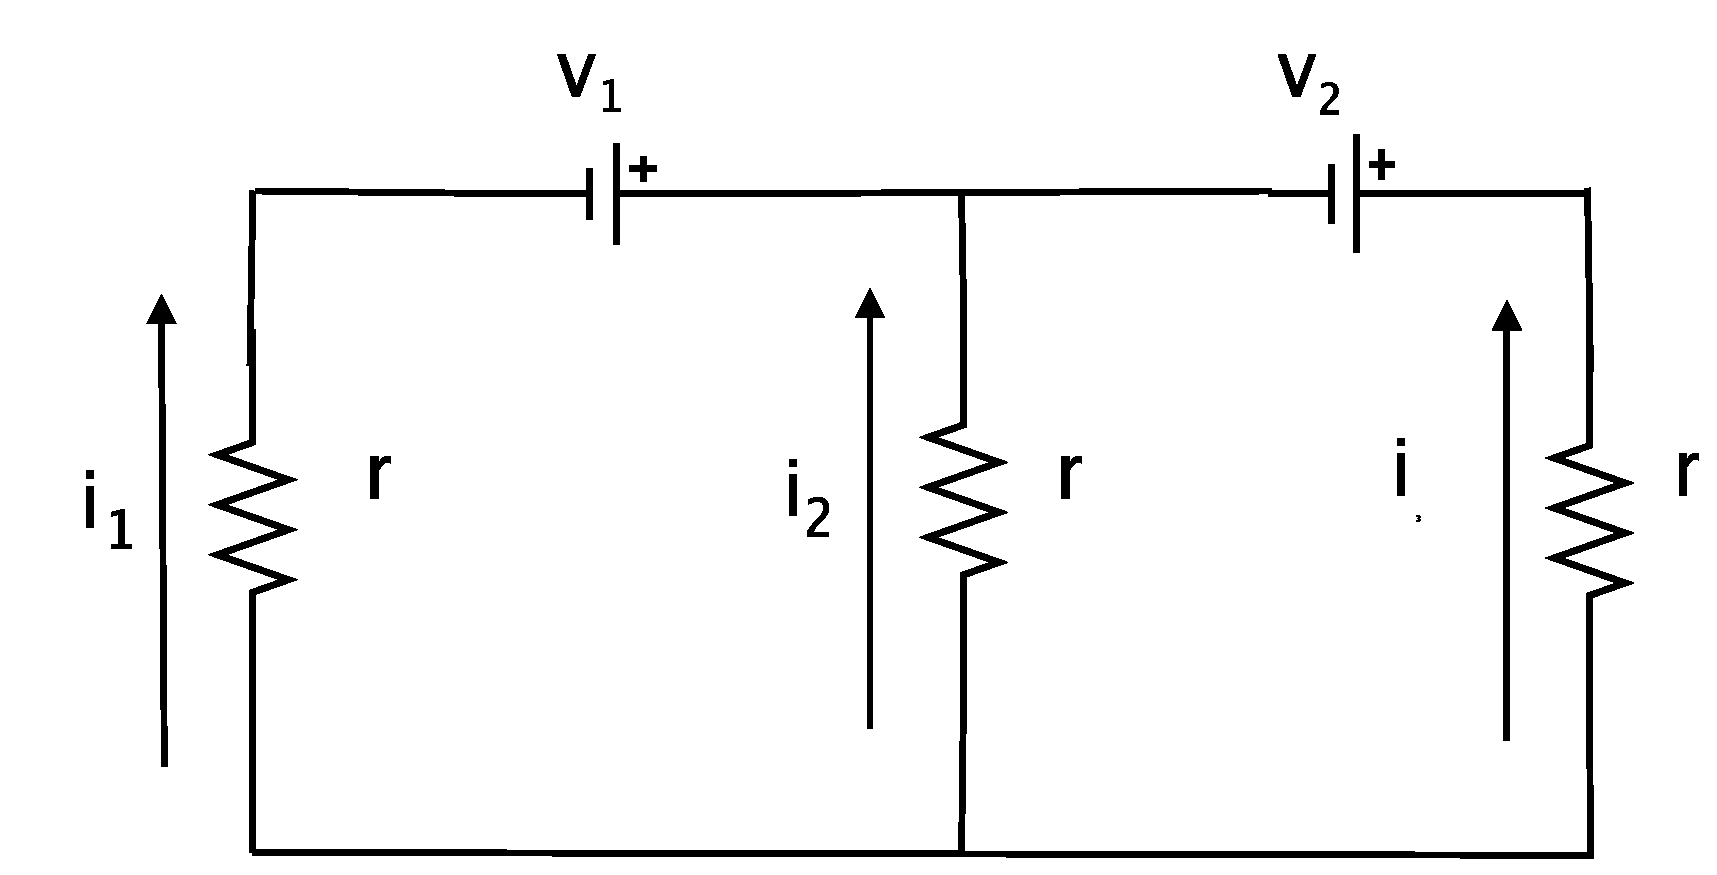
\epsfig{file=circuit.eps,width=3in}
\[ r = 14 \Omega, v_1 = 6V, v_2 = 12V \]
\begin{itemize}
\item What is the value of $i_1 r_1 - i_2 r_2$?  (Hint: you don't need
to solve for $i_1$ and $i_2$ to answer this.  $|i_1 r_1|$ is the voltage
drop across the left resistor (why?).  Remember Kirchoff's laws.)

\item What is the value of $i_1 + i_2 + i_3$?  (Hint: Look at the point
at the bottom-middle, and think about how those currents interact
there.   Make sure you think about the sign of each current.)
\item What is the value of $i_2$?  (Hint: Use the two equations from the
previous two problems.  Are those two enough equations to solve it?)
\end{itemize}

\begin{description}
\item[Main idea:]
    Basic application of Kirchoff's laws.
\item[Student process:]
    The student is probably aware that it is a Kirchoff's law problem.
A student might try to solve for the three currents first.  If
successful, then the question is answered (along with the next two).  If
not, then the hint will tell them that they don't need to solve, and
(hopefully) get them thinking more qualitiatively.

    I'm hoping for the same process in problem 2, with the student
realizing that he probably doesn't need to solve for the currents in
this case either.

    The final problem gets to the algebra.  The hint tells the student
to write down those equations.  He notices that two equations are not
enough for three variables, and then looks for another equation.
(I've observed many students flipping through their book when they need
an equation; hopefully the first problem will guide them.)
\item[Why this is an improvement:]
    I essentially thought the problem was too hard numerically.  All
I've done is to make it easier by adding more guidance.  I'm hoping to
teach the (meta-)message that a typical process is to look at a problem
to try to extract relationships (in the form of equations),
\textit{then} do math to get to the answer.  That is, separate the two
steps.  The most common error is going to be with signs, so I've
narrowed down possible errors to one equation and algebra, rather than
three equations and algebra.  This may facilitate guess-and-check
behavior with respect to signs.  It's a tough trade-off; I'd like to see
how many tries students need for the original.
\end{description}
\end{document}
